\section{Definition of Community Detection}
In the beginning, it is necessary to introduce the terminology used in this dissertation. A graph, in its intuitive understanding, is a group of nodes connected with each other to form either one connected or several disjoint components. In this thesis, a graph is also called a network, and a node or vertex (plural: vertices) is a single object appearing in the graph. The terms edge or link refers to the connections between two nodes. Graph mining, also known as complex network analysis, is the practice of exploring graphs to analyze their properties and, often, to extract them automatically. These terms are often used interchangeably, and there is no fundamental difference between them. Community detection is a subtopic within graph mining that aims to detect node closeness relationships given the graph topological structure. Also known as clustering, it entails grouping nodes into communities (also called groups or clusters) where the within-community nodes should have as many connections as possible and between-community nodes should have as few connections as possible.

Mathematically, given a graph $G(V,E)$ where $V$ is the node set and $E$ is the edge set, community detection approaches aim to find a partition $C = \{c_1,c_2,...,c_k\}$ to group all nodes into $k$ communities, where $c_i$ refers to the $i_{th}$ community with $N_i$ nodes. For the simplest scenario in which a node can only belong to one community ($v_i \in c_j$ , $N = \sum_{i=1}^k N_i$) is the number of total nodes  $|V|$ in the graph. 

A simple visualization of graph community structures is shown in Figure \ref{fig:c1_community} where nodes and edges constitute the graph and different colors refer to different communities. It is easy to see that there are three communities, which are marked in different colors (blue, green, red). Within each community, the nodes are densely connected with each other, whereas there are few edges between nodes in different communities.

The goal of community detection is to assign each node to a community (disjoint community detection) or multiple communities (overlapping community detection) in a manner that satisfies the abovementioned criteria. Apart from the simple concept definitions introduced above, a Table \ref{tab:c2_glossary} provides a comprehensive glossary of terminology used in this thesis, introducing representative symbols and brief definitions.
\begin{figure}  
	% \advance\leftskip-1cm 
	% \hspace*{0.25cm} 
	\centering
	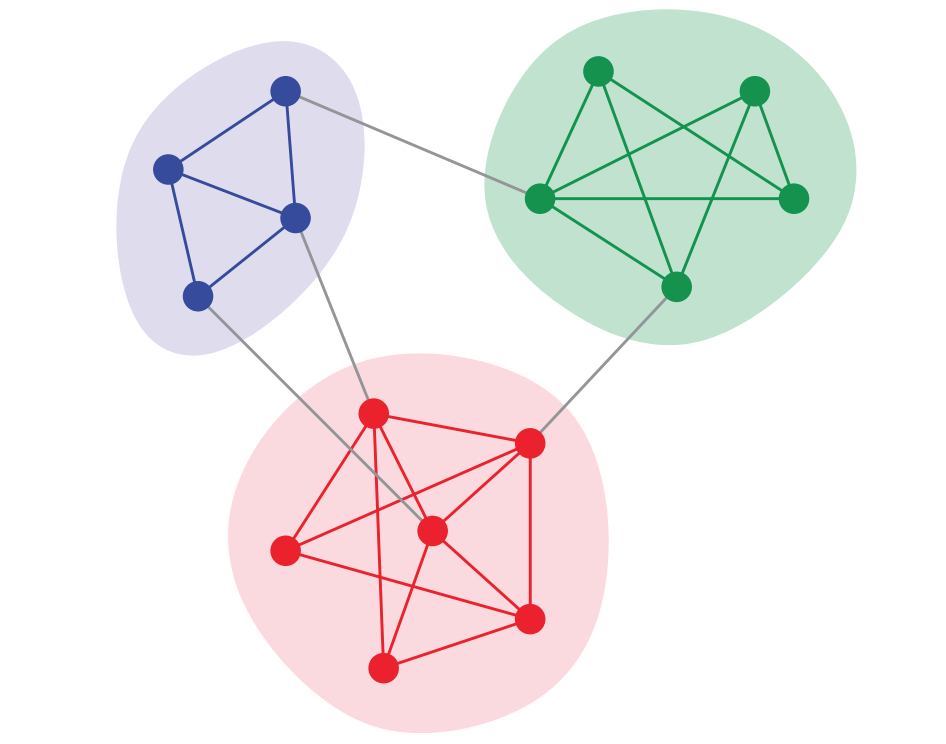
\includegraphics[width=0.5\columnwidth]{img/chapter1/community.png}
	%  \vspace{-1em}
	\caption{Example graph showing community structure. The nodes of this graph are divided into three communities, with most edges falling within communities and only a few between communities. The figure is contributed from \cite{newman2012communities}.}
	\label{fig:c1_community}
	%   \vspace{-1em}
\end{figure}
 

\begin{table}
	% \scriptsize
	\centering
	%   \vspace{-3em} 
	% \renewcommand{\tabcolsep}{2pt}
	\begin{tabular}{|p{3cm}|p{11cm}|} \hline
		\textbf{Term} &  \textbf{Definition} \\ \hline
		$G(V,E)$ & Graph $G$ with node set $V$ and edge set $E$.  \\ \hline
		$\Omega$ & $\Omega = \{ \omega_1,\omega_2,..., \omega_k\}$ is the ground truth community partition by models  where $\omega_k$ is the $k_{th}$ predicted community. \\ \hline
		$C$ & $C = \{ c_1,c_2,..., c_j\}$ is the detected community partition where $c_j$ is the $j_{th}$ community.\\ \hline
		$N, M$& $N = |V|$ denotes the node number and $M = |E|$ denotes the edge number in graph $G$\\ \hline
		$N_c$& $N_c = |c|$ is the number of nodes in community $c$\\ \hline
		$N_{c,\omega}$& $N_{c,\omega} = |c \cap \omega |$ is the common nodes in the detected community $c$ and ground truth community $\omega$ \\ \hline
		$E_{c}^{in}$& The number of edges within the community $c$. $E_{c}^{in} = \{(u,v) \in E : u \in c, v \in c \}$\\ \hline
		$E_{c}^{out}$& The number of edges on the boundary of the community $c$. $E_{c}^{out} = \{(u,v) \in E : u \in c, v \notin c$ \textit{or} $ u \notin c, v \in c \} $\\ \hline
		$D(v)$& Degree of node $v \in V$ \\ \hline
		$D_c$& The sum of node degrees in community $c$ \\ \hline
		$\mathcal{N}(v)$ & The neighbour node set of node $v$ \\ \hline
		$A$ & Graph adjacent matrix \\ \hline
	\end{tabular}
	\caption{Glossary of technical terms.}
	\label{tab:c2_glossary}
	
\end{table} 